\section{Preliminaries}
\label{sec:prelim}

In this section we introduce notation and underlying assumptions (Section \ref{subsec:notation-assume}), 
and define our observability (Section \ref{subsec:observe}) and cross-validation (Section \ref{subsec:xval-rules}) rules.

%\xx{Maybe merge Observability Rules and Cross-Validation Rules Sections}

\subsection{Assumptions, Notation, and Terminology}
\label{subsec:notation-assume}


We model a power grid as an undirected graph $G=(V,E)$.  Each $v \in V$ represents a bus. % A bus is either an electrical substation, a power generation center, or an aggregation of loads. 
$V=V_Z \cup V_I$, where $V_Z$ is the set of all zero-injection buses and $V_I$ is the set of all non-zero-injection buses.  A bus is zero-injection if it has no load nor generator \cite{Zhang10}.
All other buses are non-zero-injection, which we refer to as injection buses. Each $(u,v) \in E$ is a transmission line connecting buses $u$ and $v$. 

Consistent with the conventions in \cite{Baldwin93,Brueni05,Abur06,Mili90,Xu04,Xu05}, we make the following assumptions about PMU placements and buses. 
First, a PMU can only be placed on a bus.  Second, a PMU on a bus measures the voltage phasor at the bus and the current phasor of all transmission lines connected to it.

Using the same notation as Brueni and Heath \cite{Brueni05}, we define two $\Gamma$ functions. For $v\in V$ let $\Gamma(v)$ be the set of $v$'s neighbors in $G$, and $\Gamma[v] = \Gamma(v)\cup \{v\}$. 
A PMU placement $\Phi_G \subseteq V$ is a set of nodes at which PMUs are placed,
and $\Phi^R_G\subseteq V$ is the set of observed nodes for graph $G$ with placement $\Phi_G$ (see definition of observability below).
$k^* = \min \{|\Phi_G|:\Phi^R_G=V\}$ denotes the minimum number of PMUs needed to observe the entire network. Where the graph $G$ is clear from the context, we drop the $G$ subscript.

For convenience, we refer to any node with a PMU as a \emph{PMU node}. Additionally, for a given PMU placement we shall say that a set $W\subseteq V$ is observed if all nodes in the set are observed, and if $W=V$ we refer to the graph as \emph{fully observed}. 

\subsection{Observability Rules}
\label{subsec:observe}

We use the simplified observability rules stated by Brueni and Heath \cite{Brueni05}. For completeness, we restate the rules here:
\begin{enumerate}
	
	\item {\bf Observability Rule 1 (O1)}.  {\it If node $v$ is a PMU node, then $v \cup \Gamma(v)$ is observed. } %Formally, if $v \in \Phi_G$, then $\Gamma[v] \subseteq \Phi^R_G$. }

	\item {\bf Observability Rule 2 (O2)}. {\it If a zero-injection node, $v$, is observed and  $\Gamma(v)\backslash\{u\}$ is observed for some $u\in\Gamma(v)$, then $v \cup \Gamma(v)$ is observed.}
	%Formally, if $v \in \Phi^R_G \cap V_Z$ and $|\Gamma(v) \cap (V - \Phi^R_G)| \leq 1$, then $\Gamma[v] \subseteq \Phi^R_G$. }

\end{enumerate}

Consider the example in Figure \ref{fig:pmu-example}, where the shaded nodes are PMU nodes and $g$ is the only zero-injection node. 
Nodes $a-d$ are observed by applying O1 at the PMU at $a$, and nodes $a,b,f$ and $g$ are observed by applying O1 at $b$. 
$e$ cannot be observed via $c$ because $c$ does not have a PMU (O1 does not apply) and is an injection node (O2 does not apply). 
Similarly, $j$ is not observed via $f$. Finally, although $g \in V_Z$, O2 cannot be applied at $g$ because $g$ has two unobserved neighbors $i,h$, so they remain unobserved.

Since O2 only applies with zero-injection nodes, the number of zero-injection nodes can greatly affect system observability. 
For example, consider the case where $c$ and $f$ are {\em zero-injection} nodes. $a-d$, $g$ and $f$ are still observed as before, as O1 makes not conditions on the node type. Additionally, 
since now $c,f \in V_Z$ and each has a single unobserved neighbor,  we can apply O2 at each of them to observe $e,j$, respectively. % making $e$ and $j$, respectively, observed.   
We evaluate the effect of increasing the number of zero-injection nodes on observability in our simulations (Section \ref{sec:simulations}).


\begin{figure}[t]
\centering
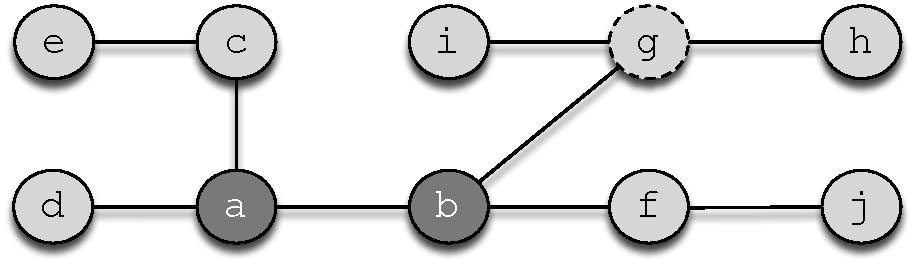
\includegraphics[scale=.6]{figs/pmu-example.pdf}
%\includegraphics[scale=0.51]{figs/example2.pdf}
\caption{Example power system graph. PMU nodes ($a,b$) are indicated with darker shading. Injection nodes have solid borders while zero-injection nodes  ($g$) have dashed borders.}
\label{fig:pmu-example}
\end{figure}

\subsection{Cross-Validation Rules}
\label{subsec:xval-rules}

Cross-validation formalizes the intuitive notion of placing PMUs ``near'' each other to allow for measurement error detection. 
From Vanfretti et al. \cite{Vanfretti10}, PMU measurements can be cross-validated when: (1) a 
voltage phasor of a non-PMU bus can be computed by PMU data from two different buses or (2) the current phasor of a transmission line can be computed from PMU data from two different buses. 
{\footnote {Vanfretti et al. \cite{Vanfretti10} use the term ``redundancy'' instead of cross-validation. }  


%`A PMU node is cross-validated if {\em the PMU node is within two hops of another PMU node}. 
For convenience, we say a PMU is cross-validated even though it is actually the PMU data at a node that is cross-validated.
A PMU is \emph{cross-validated} if one of the rules below is satisfied \cite{Vanfretti10}: 
%More formally, a PMU is \emph{cross-validated} if one of the rules below is satisfied \cite{Vanfretti10}: 
\begin{enumerate}
	
	\item {\bf Cross-Validation Rule 1 (XV1)}.  {\it If two PMU nodes are adjacent, then the PMUs cross-validate each other. }
	%Formally, if $u, v \in \Phi_G$, $u \in \Gamma(v)$, then the PMUs at $u$ and $v$ are cross-validated.}

	\item {\bf Cross-Validation Rule 2 (XV2)}. {\it If two PMU nodes have a common neighbor, then the PMUs cross-validate each other.}
	%Formally, if $u, v \in \Phi_G$, $u\neq v$ and $\Gamma(u)\cap\Gamma(v)\neq\emptyset$, then the PMUs at $u$ and $v$ are cross-validated.}
\end{enumerate}
In short, the cross-validation rules require that {\em the PMU is within two hops of another PMU}.
For example, in Figure \ref{fig:pmu-example}, the PMUs at $a$ and $b$ cross-validate each other by XV1.

XV1 derives from the fact that both PMUs are measuring the current phasor of the transmission line connecting the two PMU nodes.  XV2 is more subtle.  
Using the notation specified in XV2, when computing the voltage phasor of an element in $\Gamma(u)\cap\Gamma(v)$ the voltage equations include variables to 
account for measurement error (e.g., angle bias) \cite{Vanfretti-thesis}. 
When the PMUs are two hops from each other (i.e., have a common neighbor), there are more equations than unknowns, allowing for measurement error detection. 
Otherwise, the number of unknown variables exceeds the number of equations, which eliminates the possibility of detecting measurement errors \cite{Vanfretti-thesis}.





